\documentclass[conference]{IEEEtran}

\usepackage[dvips]{graphicx}
%\usepackage{graphicx}
\usepackage{amsmath,amssymb}
\usepackage{algorithm}
\usepackage{algorithmic}
\usepackage{subcaption}

\begin{document}
\title{Investigating Networked Music Performances in Pedagogical Scenario for the InterMUSIC Project}
%\title{Paper Title (Each Word of the Title Should Begin with a Capital Letter with the Exception of Articles and Conjunctions)}
\date{}%date stay empty

\author{
\IEEEauthorblockN{Luca Comanducci, Michele Buccoli,\\ Massimiliano Zanoni, Augusto Sarti}
\IEEEauthorblockA{DEIB, Politecnico di Milano  \\ Milan, Italy \\ \{name.surname\}@polimi.it\\}
\and
\IEEEauthorblockN{Stefano Delle Monache\\ }
\IEEEauthorblockA{Dept. of Architecture and Arts \\ Iuav University of Venice \\sdellemonache@iuav.it\\}
\and
\IEEEauthorblockN{Giovanni Cospito, Enrico Pietrocola, \\Filippo Berbenni}
\IEEEauthorblockA{Conservatory of Music G. Verdi of Milan \\ Milan, Italy \\ \{name.surname\}@polimi.it\\}}


\maketitle


\begin{abstract}
With the big improvement of digital communication networks, Networked Music Performances (NMP) received a great interest from music live performance e music recording industry. The positive impact of NMP in pedagogical applications, instead, it has been only preliminary explored. Within the InterMUSIC project, we aim to investigate NMP from a pedagogical perspective, that has considerable differences with respect to music performances, and to develop tools to improve distance learning experiences. In this paper, we introduce a conceptual framework designed to be the foundaments for all the experiments conducted in the project. We also present two preliminary experiments that investigates on the sense presence of geographically-distant musicians in distance learning scenario. We discuss the comments provided by the musicians as a set of requirements and guidelines for future experiments.
\end{abstract}


\section{Introduction}\label{sec:introduction}

The rapid evolution of technology and the consequent increasing speed of digital communication networks allows to improve the communication experiences with the dramatically reduction of the virtual distances. Among the others, the process, facilitates the emerging of new scenarios of interaction among geogra\-phically-displaced people. Since the late '90s, a community composed of musicians, technicians and  scientists has been investigating how technology can enable music performances leading to the definition of Networked Music Performance (NMP), which \textit{occurs when a group of musicians, located at different physical locations, interact over a network to perform as they would if located in the same room} \cite{Lazzaro2001}.

NMP has immediate application in the performative scenario, enabling musicians to rehearse from remote distances and to perform in geographically-distributed concerts \cite{barbosa2003displaced}. As part of the broader category of audio-video streaming and conferencing systems, NMP has been interesting applications of educational purpose such as blended and distance learning \cite{IorwerthNMP2015}.    


% InterMUSIC: what it is, what it aims, how it is involved with NMP.
The EU funded project InterMUSIC\footnote{http://intermusicproject.eu/} (Interactive Environment for Music Learning and Practicing, 2017 - 2020) aims to develop and improve tools for distance learning of music and to collect such tools in integrated remote environments for music interaction and education. Within the project we have chosen three online pilot courses: music theory and composition, chamber music practice, and vocal training. Tools for courses are developed following two main paradigm. %Tools for course are developed by means of 

In the first paradigm, students from any part of the world access the course and find the teaching material provided by the teacher, with the possibility to interact with their colleagues and professors. This paradigm, namely Massive Open Online Courses, is designed for one-to-many asynchronous communication and it is widely used also by elite universities \cite{MOOCS}.

In the second paradigm, students use NMP softwares for attending master-student lessons or rehearse together. This paradigm has stricter requirements in terms of synchronicity and therefore only allow one-to-one (or few-to-few) synchronous communication. In this paper, we focus on the NMP-based paradigm and we discuss the  requirements related to the specific pedagogical scenario.

%Music Networked Performance is an interesting outcome of technology, and has receive attention under different factors.
The literature about NMPs has investigated numerous factors which may affect several aspects of the performances. Affecting factors include the unavoidable network latencies \cite{Chafe1}, timbral properties of the employed instruments \cite{Kolazi2013} and rhythmic properties of the performed pieces \cite{RottondiFeature}; while affected aspects range from objective quality of the performance \cite{Chafe3}, to perceptual metrics of musicians' comfortability \cite{CIM2018}. This investigation has led a highly popular tool for NMP, which allows low-latency interaction by using high-end hardware connected through ad-hoc inter-university network \cite{drioli2013networked}. 

%  For pedagogical applications, however, may involve other factors, such as the quality of sound, the sound environment, the spatial acoustics information.
In order to widen the audience of NMP, it needs to be available also for general purpose connections and hardware, hence addressing higher processing and transmission latency. Nevertheless, with the idea of using NMPs in the educational context, the goal of is not the NMPs' objective or subjective quality, but rather on those aspects and factors that can guide students to improve their technique or enable comfortable remote rehearsal. 

% we do not know which aspect to investigate--> we need experiments
The aspects we need to address for the success of pedagogical NMPs are not known a priori, leading us to make some assumptions. For example, we may assume that the acoustics of the environments affect or alienate the sense of presence of performers, or we may require that the networked environment should not worsen students' level of stress. In order to verify our assumptions, we need to conduct perceptual experiments with musicians to test different conditions and evaluate the result of these experiments. Back to the previous examples, we need to test how musicians perform in environments with different acoustics, or we need to measure musicians' stress level using sensors for biometric signals \cite{Yoshie2009}. While conducting these experiments, we also want to start an open dialog with music teachers and students to collect comments during the performances and translate them into technical requirements for the project. 

With this goal in mind, in this paper we identify the main entities involved in the performances and the interaction among them and we formalize them in a framework. The role of the framework is to provide an abstraction for the experiments that we need to conduct. The framework is designed to be generic for any kind of networked or physical performance, and we plan to extend it in order to provide a comprehensive semantic description of rehearsal and teaching activities for pedagogical scenarios. We present the architecture and details of the framework in Section \ref{sec:framework}.

Using this framework, we are able to design the perceptual experiments for conducting investigations on NMPs in the pedagogical scenarios. In Section ~\ref{sec:setup} we describe two pilot experiments we conducted to investigate the role of visual cues in musical interaction, and the influence of latency in the sense of presence of musicians, respectively. The preliminary results of the experiments and the next steps of our investigation are presented in  Section \ref{sec:discussion}.  

%on the temporal factors. We discuss the outcome of these tests in terms of preliminary perceptual and objective results and highlighting those comments from students that will guide our future work with the project.


%Moreover, we must continue to take the influence of latency into consideration to correctly design our tools for NMP.

%On the one side, we need to take the influence of latencies into consideration  This involves to conduct perceptual tests to understand how these temporal factors affect the sense of presence, and the quality of the performance. On the other side, we also aim at 


%In this paper, we present the architecture of the framework we will use for the perceptual tests and we describe the tests we have conducted on the temporal factors. We discuss the outcome of these tests in terms of preliminary perceptual and objective results and highlighting those comments from students that will guide our future work with the project.

%The paper is organized as follows: in Section~\ref{sec:background} we provide the background context on top of which we are building our study; in Section~\ref{sec:framework} we present the designed architecture for perceptual experiments;  steps of the project in Section~\ref{sec:discussion}.

%In this paper, we introduce a study, still in progress, aimed at understanding how temporal factors (i.e., network latency) affect the sense of presence, and the quality of the performance of chamber music duos involved in remote collaboration, i.e music making. 
%
%We ask duos to perform a short exercise, under diverse conditions of network delay. 
%The exercise is specifically conceived around musical structures which are functional to pinpointing a set of problems relative to time management, communication mechanisms and mutual understanding between remote performers. A qualitative assessment through questionnaires on the sense of presence and the perceived quality of the performance~\cite{schubert2001experience} is combined with quality metrics of the objective performance~\cite{rottondi2015feature}.
%A follow-up study will be devoted instead to the investigation of spatial representations, auditory and visual.
%
%The premise is that effective music-making and communication rely on the availability of auditory and visual cues (i.e., sonic gestures)~\cite{godoy2010musical}, which are inevitably constrained in NMP, and in telepresence environments in general. 
%We turn the traditional engineering approach to NMP research upside down, and seek for design strategies to compensate, and facilitate a plausible music experience in the mediated environment. 
%
%In this respect, we are investigating how simulated network delay, and diverse modes of audio-visual spatial representation, separately, affect the subjective experience of being present and together in the shared reality environment. 
%Sensory breadth and depth, degree of control and anticipation of events, together with the overall interactivity of the environment, represent crucial elements in both presence and performance, being the first a prerequisite for the second~\cite{nash2000review}.
%


\section{Background and Related Work}\label{sec:background}
A wide investigation on NMPs has been devoted to the influence of different latency conditions on the performance. We discuss the main results in Section \ref{subsec:temporal}. In Section \ref{subsec:network} we briefly introduce the investigation regarding the network topologies and architecture, while in Section \ref{subsec:acoustics} we provide an overview of the studies on rooms' acoustic factors. Lastly, in Section \ref{subsec:sw} we list the main softwares employed for NMPs and their main features.

\subsection{Temporal factors}\label{subsec:temporal}
Temporal factors refer to every aspect of the infrastructure that cause the presence of end-to-end delay between the musicians present in different locations. We can broadly divide the causes of end-to-end delay into two main factors, i.e., the signal processing delay and the network delay \cite{Lakiotakis}. 

The former comprises the delays caused by the whole signal chain, consisting of acquisition hardware (e.g. soundcards), the encoding/decoding and fragmentation processes. The latter comprises all the possible delays caused by the network transmission between transmitter and receiver due for example to network congestion.

The level of latency is a factor that dramatically affects the NMP experience and as such was extensively analyzed in the literature. In~\cite{RottondiFeature} the authors conduct a series of content-based experiments that show how high latency values in the range of $20-60~\mathrm{ms}$ cause a decrease in the quality of the performance expressed by a tendency of the musicians to tempo deceleration. 

In~\cite{Chafe1,Chafe2,Chafe3} the authors take into account the concept of \textit{Temporal Separation}, which represents the time needed for the action of one person to reach another one in a setting where both are acting together. A set of experiments are devised, which evaluate the ability of several couples subjects in performing a clapping rhythm together while being in two separated rooms and while varying the transmission latency in the range of 3-78 ms. The results of such experiments prove that the best performance results are obtained when the transmission latency between the subjects is comparable to a Temporal Separation value corresponding to a setting where the two subjects are in the same room. The authors also observed that unnaturally low latency values cause an acceleration in the musicians' tempo.

%When confronted with latency values different from a \textit{Temporal Separation} corresponding to a physical setting, the musicians devise a set of techniques in order to cope with such difficulty. Such techniques are identified in~\cite{Carot07networkmusic} and vary depending on the latency level. If the latency is less than $25\mathrm{ms}$ the musicians are able to follow a Realistic Interaction Approach (RIA), which corresponds to the delay that would have been sensed if they were in the same room. This is the only type of approach considered acceptable for professional musicians. When latency exceeds $25\mathrm{ms}$ the subjects find different ways to cope with latency, depending on the scenario and on the type of music. In the Master Slave (MSA) and Laid Back (LBA) approaches one of the two musicians follows its own tempo, while the second one follows. MSA is appropriated when two rhythm instruments are performing, since one can simply follow the rhythm of the other, instead, in the case of LBA we usually have a rhythmic and solo instrument playing, the rhythmic one mantains the tempo, while the solo one performs slightly out of time. The Delayed Feedback approach tries to make the musicians as if they were in a RIA setting, by delaying artificially the signal of one of the players.

\subsection{Network factors}\label{subsec:network}
The choices regarding all the aspects of the network architecture depend on the aspects needed in the NMP framework. 
Network architecture used for NMP comprise both decentralized peer-to-peer(P2P) and client-server~\cite{RottondiOverview}. 

In P2P architectures each participant has to send its audio/video data to all the other musicians. This poses great issue for what concerns the scalability of the NMP system, causing a trade-off between the number of people connected and the quality of the audio-video content, which must be degraded in order to gain enough bandwidth to connect all the musicians.

Client-server architectures address the scalability issue, since they are based on a server that receives the individual streams sent by each musicians, mixes it and then sends it back. However, the bandwidth requirements remain rather high, and the server causes an additional delay, since it adds a two-way communication with each participant.


\subsection{Acoustic and Spatial factors}\label{subsec:acoustics}
The analysis of the impact of acoustic and spatial factors in NMP and distance learning has not been as deep and thorough as the ones performed on the analysis of the tempo effects. 

%The effect of the acoustic environment were considered in few works. 
In~\cite{carot2009towards} the authors performs a set of experiments in semi-anechoic chambers and add different levels of artificial reverb in order to simulate a natural environment. The experiments show that the performances of the musicians provide no noticeable differences that could be directly explained by the change in reverberation. 

In \cite{FarnerReverb}, the author present an experiment with two musicians performing handclapping (similarly to \cite{Chafe1}) considering three acoustic conditions: real reverberant, virtual anechoic and virtual reverberant. The results show that anechoic conditions cause higher imprecisions than the reverberant ones.

In~\cite{gurevich2011ambisonic} the authors present a study that concerns the application of Ambisonics techniques to NMP problems. Athough they do not develop a fully functional framework for NMP, they demonstrate the feasibility of implementing 3D spatial audio for NMP tasks. %which may be one of the field most future developments.


\subsection{Available softwares}\label{subsec:sw}
In this Section we list the main tools that have been developed for NMP; for an extensive list we refer the reader to ~\cite{RottondiOverview}.

JackTrip~\cite{CaceresJacktrip} was developed by the SoundWIRE research group at CCRMA in order to support bi-directional music performances. It is based on uncompressed audio transmission through high-speed links such as \textit{Internet2}. In the current version, it does not support video transmission.

The LOLA\cite{drioli2013networked} project was developed by the Conservatory of Music G. Tartini in Trieste in collaboration with the Italian national computer network for universities and research (GARR). LOLA is based on low-latency audio/video acquisition hardware and on the optimization of all the steps needed to transmit audio/video contents through a dedicated network connection. Because of  its low-latency properties, we used it in the preliminary InterMUSIC experiments presented in \cite{CIM2018}. As a drawback, the project is not open source and it is not optimized for generic network connections.

On the other side, UltraGrid~\cite{holub2006high} is an open-source software that allows audio/video low latency transmission. While its performance are still far from those achieved by LOLA, it is more flexible for generic hardware and networks and it allows contributors to implement  new functionalities. For this reason, we are considering the use of UltraGrid in the next stages of the InterMUSIC project.
\section{Framework}\label{sec:framework}
%\textbf{MANCA UNA INTRO MOTIVANTE DELLO SCHEMA}\\
%Considering the aforementioned requirements, we designed the conceptual framework that employed conducting perceptual experiments. We identify the following entities that are in relation to each other in numerous ways. 
In this Section, we introduce a framework for the design of perceptual experiments on musical performances. The framework is composed of five main entities, which interact with each other in numerous ways, depending on the kind of experiment we want to conduct and performance we aim to observe. The framework can be considered as a first formalization of the problem of investigating NMP, and we aim to develop it further during the project.

We show in Fig. \ref{fig:framework} a schematic representation of the framework and the basic relations among entities. A \textbf{performance} occurs when two or more \textbf{subjects} musically interact together through a \textbf{medium}. Subjects can be musicians during a rehearse, as well as teachers and students. In order to consider a large number of probable scenarios, a performance can occurs with all the subjects in the same room (\textit{local performance}), with all the subjects geographically distant (\textit{networked performance}) or with part of the subjects in the same place and part of the subjects geographically distant (\textit{mixed performance}). Subjects interact by means of a \textit{medium}. In the case of local performances, the medium is a \textit{physical medium}, such as simple air propagation. In the case of networked performances, the medium is \textit{networked medium}, such as an Internet connection and the NMP software/hardware equipment to connect the two subjects. In the case of mixed performance the both physical medium and networked medium are involved. 

In all the scenarios subjects performs in an \textbf{environment} with specific timbral (acoustic of the room) and spatial properties (location of the subjects in the room). In the case of networked and mixed performance, environments with different characteristics are potentially involved. Given a subject, we define the environment he/she playing as the \textit{real environment} and the environment they perceive of the geographically-distant subjects as the \textit{virtual environment}. For example, in Fig. \ref{fig:afsv}, we show a set of frames from one of the experiments we conducted. Fig. \ref{subfig:as} shows a harp player in her \textit{real} environment; her partner's perception of this environment, i.e., the \textit{virtual environment}, is shown in Fig. \ref{subfig:av}. 

%Since the investigation of the sense of presence is one of the main goals of the experiments, the study of the interaction between the real environment with the virtual environment is crucial. This 

%\textbf{DIRE QUALCOSA IN PIU\' DI QUALI ELEMENTI ENTRANO IN GIOCO}.

%the environments are different, the subjects will interact through a \textit{networked medium}, hence having a NMP; otherwise they interact through a \textit{physical medium}. The comparison between a networked and physical medium is crucial to understand how to design the interaction so that the \textit{virtual environment} perceived from the other end of the medium matches the expectations of a real environment. 

In order to analyze the performance, it is crucial to run a \textbf{data recording} stage, using different devices to capture the multimodal signals. The factors and aspects that will be possible to analyze from the performance depend on the properties of the devices, e.g., whether they are \textit{video} or \textit{audio devices}, or where they are placed. In the following sections we describe in detail the aforementioned entities.



\begin{figure}[t]
	\centering
	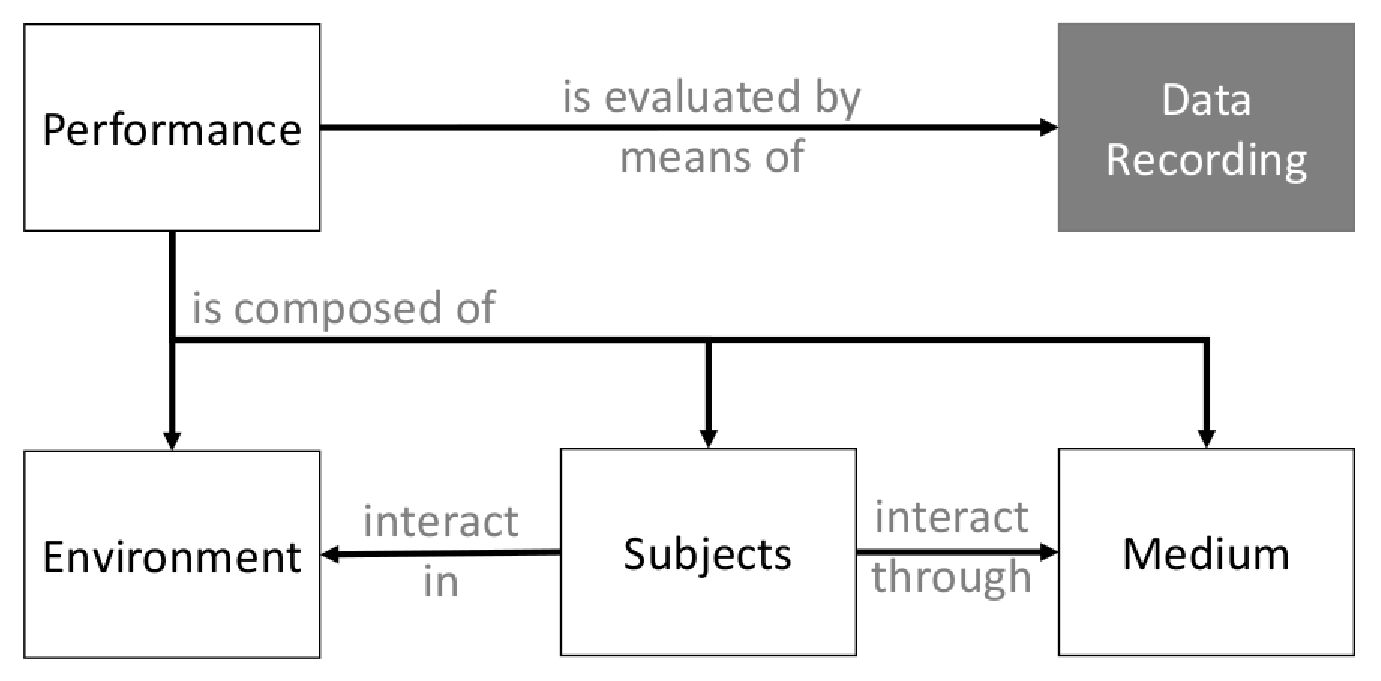
\includegraphics[width=\columnwidth]{img/framework.eps}
	\caption{A graphical representation of the proposed framework with main entities and interaction.}
	\label{fig:framework}
\end{figure}

\subsection{Performance}
In our experiments we consider two types of performances: \textit{performed piece} or \textit{taught lesson}. The performance is the entity at the highest hierarchical level and it is composed of the subjects, the environments and the mediums. 
Main properties of the performance are date and time, location(s), types of performance, such as is better detailed in the subjects' \textit{part} property, metadata (e.g., composer of the piece, tempo, meter, key signature, score, duration, etc.) and composition  description in form of symbolic representation (MIDI or musicXML) \cite{MIDItoolbox}.

Some properties of the performance depend on the nature of its sub-entities. For example, if the subjects are two musicians, the performance can be a \textit{rehearsal} or a \textit{concert}, while if one of the subject is a teacher, the performance is defined as a \textit{lesson}. As discussed above, the property of performance also depends on the type of medium: we have a networked or mixed performance if we have at least one networked medium.   

\subsection{Subjects}
Subjects are involved in the performance with different possible roles, such as musicians, students, teachers or conductors. Subjects are identified with their name, age, experience, musical background, that evolve over time and so must be referred to the day of the performance. Other properties inherently related to a subject is the assigned part -what they are performing- and the used instrument. These two properties can be also described by means of a content-based analysis of their musicological (e.g., rhythmic complexity) or timbral (e.g. attack time) properties, respectively \cite{RottondiFeature}.
Doing this, it is possible to analyze how such properties as aspects that may affect the final quality or success of the performance.


\subsection{Environment}
We refer to the spatial and acoustic properties of both the physical place where a subject performs and the perception of it by the other subjects as physical and virtual environment, respectively. The properties of the virtual environment depend on the location and specifics of the audio/video capture and rendering devices, such as the microphone and speakers connected to the NMP equipment. For example, using an array of microphones we can capture the acoustic scene~\cite{Markovic2013} and render it using arrays of speakers through spatial audio techniques~\cite{bianchi2016}.

Properties of the environment are also the possible processing applied to the audio or video signals. For example, by applying a reverb to the incoming audio signal, a subject will have a different perception of the virtual enviornment.

We also collect the information about the interaction of the subjects with the environment, such as the position of the musicians in the room, the details of the audio/video acquisition (e.g., microphone on the instrument vs. fixed position microphone) and the relative position of musician and devices. 

\subsection{Medium}
The medium refers to the connection between the environments and, hence, the subjects. In case of a networked performance, the medium collects the information on the employed software for NMP and its settings, the network architecture and specifics, like bandwidth, latency. In case of a performance in the same room, like a traditional lesson, we collect information as the distance between the subjects, which measures the acoustic latency between them, and describe possible visual / acoustic occlusion that may be placed between the musicians. 


\begin{table}
	\centering
	\caption{Details of the experiment in co-presence}
	\begin{tabular}{p{1.5cm}p{6cm}}
		\hline
		\textbf{Entity} & \textbf{Properties} \\
		\hline
		\textbf{Performance} & Co-presence performance. \newline Parts arranged from Bartok pieces as described in [cit]. \\
		\textbf{Subjects} & Two brothers, violin and cello players. \newline Violin player: male, 25 years, 17 years musical experience; 	\newline Cello player: male, 19 years, 10 years  musical experience \\
		\textbf{Environment} & Recording and mastering studio in the Conservatory of Milan; acoustically equipped with bass traps. \newline Musicians sit side by side, with peripherical vision.\\
		\textbf{Medium} & Condition 1: Air propagation. \newline Condition 2: Visual occlusion applied by means of a a screen with progressive layers of canvas applied to decrease transparency and visibility. \\
		\textbf{Data} \newline \textbf{recording}  & Interview to the participants and free comments.\\
		\hline
	\end{tabular}
	\label{tab:exp1}
\end{table}


\subsection{Data recording}
In order to observe the experiment and draw meaningful conclusions, we need to record the properties of the performance that are interesting for our analysis. For the data recording stage, we consider multimodal signals and their processing byproduct as well as questionnaire filled by the subjects. In the former case, we can extract objective metrics of the performance, while in the latter we consider subjective results; both are important to assess the outcome of the experiment. 

With regard to the multimodal signals, the audio recording of the performance, from the two environments, are clearly useful to assess the quality of the performance or possible modifications in the timbral or rhythmic properties. Beyond that, video recordings are also useful to annotate saccadic movement during the interaction between the subjects \cite{vandemoortele2018gazing}, and we aim to capture biometric signals to objectively estimate the subjective distress of the performers \cite{Yoshie2009}. 



\section{Preliminary experiments}\label{sec:setup}
In this Section, we describe two preliminary experiments we conducted in Spring 2018 following the conceptual framework presented in the previous section. The first experiments is a rehearsal between two musicians in the same room, where we insert visual occlusions to test their ability to interact in adverse conditions. The second experiments is a set of rehearsals between five couples of musicians in two separate rooms, connected via a network emulator to test the sense of presence and the quality of performance at different latency conditions. The results of the two experiments are discussed in the next section.


\begin{figure}[t]
	\centering
	\includegraphics[width=\columnwidth]{img/veli.eps}
	\caption{The two musicians in experiment 1, with partial occlusion and blurred effect.}
	\label{fig:veli}
\end{figure}

\subsection{Co-presence performance with visual occlusion}
We invited a string duo to make a pilot test of the environment, the perceptual questionnaire and the musical pieces that we intended to use for the second experiment. We also included a test on adverse conditions of the medium (visual occlusion) to qualitatively assess the importance of video feedback in NMPs.

We show a summary of the test conditions in Table \ref{tab:exp1}. The two subjects were a violin and a cello players and are brothers, they have a long-time experience playing together and use a wide set of visual and audio cues to interact. For the musical parts, we created a composition that requires mutual interaction and understanding. The composition includes attacks, alternate scales, changes of tempo, unison playing, sustained loop. The parts are described in detail in \cite{CIM2018} and publicly available\footnote{https://tinyurl.com/intermusicCIM2018}.


\begin{figure*}[t]
	\centering
	\begin{subfigure}[t]{.48\columnwidth}
		\centering        
		%\includegraphics[trim={.5cm 13.7cm 13.5cm .5cm},clip,width=\textwidth]{figures/ann1}
		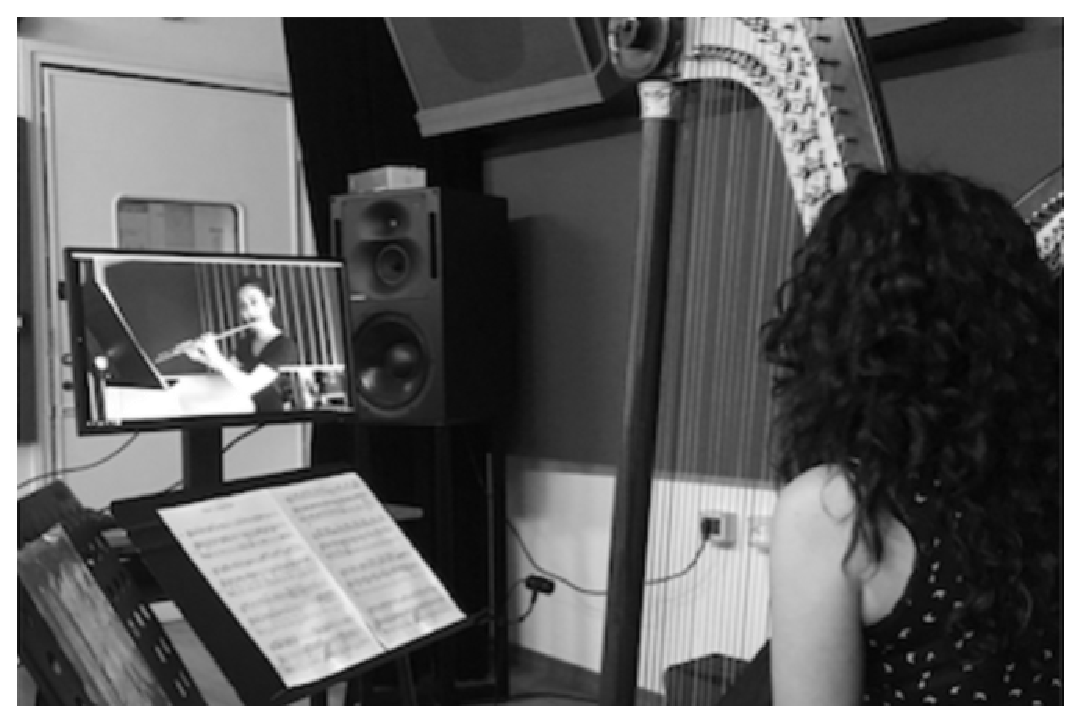
\includegraphics[width=\textwidth]{img/as.eps}
		\caption{A harp player performing in her real environment}
		\label{subfig:as}
	\end{subfigure}
	\begin{subfigure}[t]{.48\columnwidth}
		\centering        
		%\includegraphics[trim={.5cm 13.7cm 13.5cm .5cm},clip,width=\textwidth]{figures/ann1}
		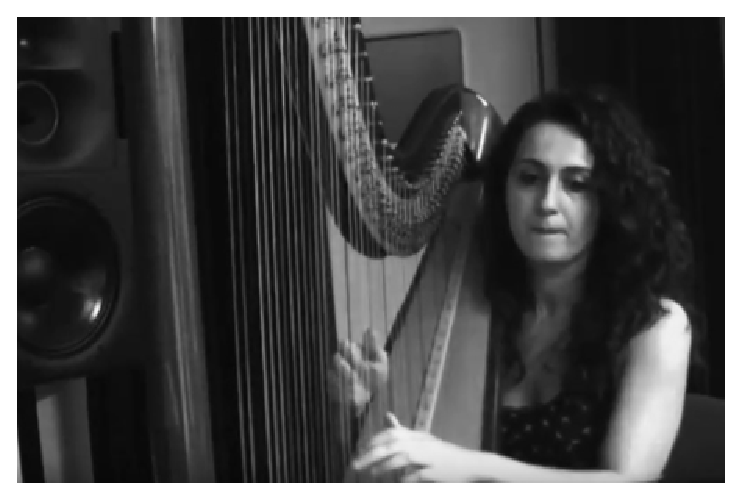
\includegraphics[width=\textwidth]{img/av.eps}
		\caption{A harp player as visually perceived in the virtual environment}
		\label{subfig:av}
	\end{subfigure}
	\begin{subfigure}[t]{.48\columnwidth}
		\centering        
		%\includegraphics[trim={.5cm 13.7cm 13.5cm .5cm},clip,width=\textwidth]{figures/ann1}
		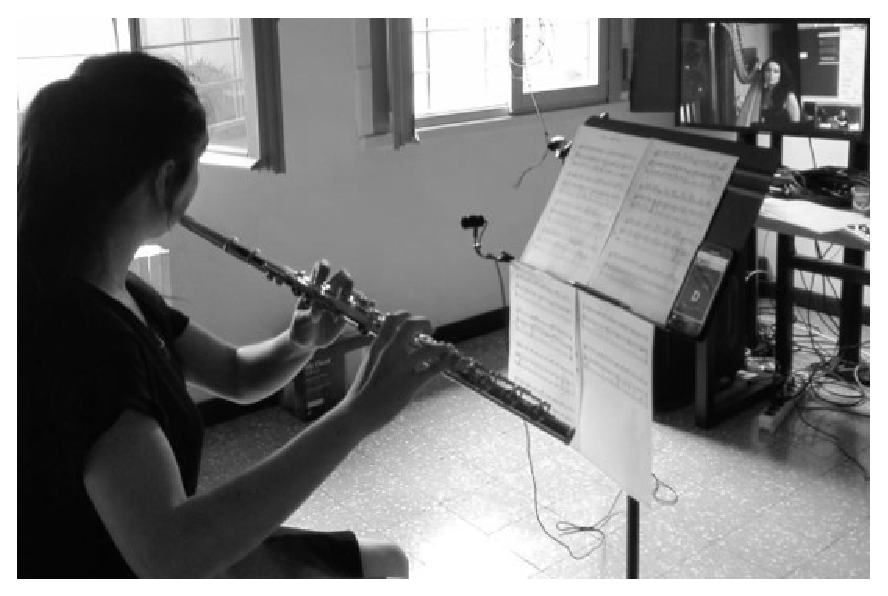
\includegraphics[width=\textwidth]{img/fs.eps}
		\caption{A flute player performing in her real environment}
		\label{subfig:fs}
	\end{subfigure}
	\begin{subfigure}[t]{.48\columnwidth}
		\centering        
		%\includegraphics[trim={.5cm 13.7cm 13.5cm .5cm},clip,width=\textwidth]{figures/ann1}
		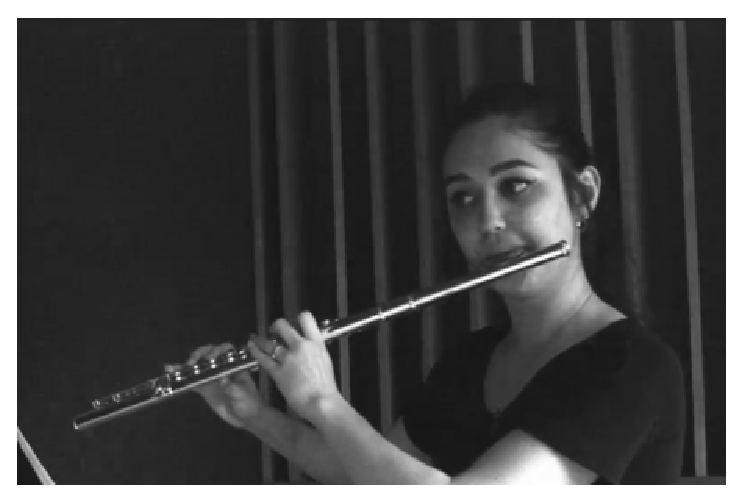
\includegraphics[width=\textwidth]{img/fv.eps}
		\caption{A flute player as visually perceived in the virtual environment}
		\label{subfig:fv}
	\end{subfigure}
	
	\quad 
	\caption{View of real environments and virtual environments in the networked experiment}\label{fig:afsv}
	
\end{figure*}

The performers were asked to play in two conditions: with no visual occlusion, and with partial visual occlusion, by inserting a tulle panel between the two instrumentalists, thus providing a blurring effect on their figures (as shown in Fig. \ref{fig:veli}). The aim was to observe their behavior, adaptation strategies, and emerging non-verbal communication (bodily and musical gestures).

The data recording of the experiment was based on a subjective questionnaire on their sense of presence and free comments on the experience. 





\subsection{Sense of presence in NMPs}
Five couples of musicians, playing different combinations of instruments, took part in the experiment. The couples had familiarity in playing together since at least two weeks. The details of the experiment are reported in Tab.~\ref{tab:exp2}

Each session of the experiment comprised a single couple, the two musicians were placed in different rooms, standing in front of a screen, in order to be connected both with respect to video and audio. An example of the setup for the couple consisting of harp and flute players is shown in Fig.~\ref{fig:afsv}. In Fig.~\ref{subfig:as} and Fig.~\ref{subfig:fs} it is possible to see the viewpoints of the musicians consisting of the scores and the screens connected to the other room. 

The couples played the same parts considered in the previous experiments. The medium involved two computers equipped with LOLA connected through a network emulator, by means of which we could change the transmission latency. A single session consisted of the couple playing the same part in six repetitions, where each time we simulated a different latency level in a range between $28\mathrm{ms}$ and $134\mathrm{ms}$, as detailed in~\cite{CIM2018}. It is important to note that the latency levels weren't presented sequentially to the musicians (e.g. in a decreasing or increasing order), but were instead selected with no particular criterion for each repetition,.

We asked the musicians to fill two different subjective questionnaires. The first one was presented after each repetition and composed of five questions, selected in order to analyze their perception of the performance with respect to the latency just experienced. The second, reported in \cite{CIM2018}, was presented to the musicians at the end of the whole session and it consisted on a 27 questions, investigating he various aspects of the experience such as their sense of presence and the peceived general quality of the performance.


\begin{table}[b]
	\centering
	\caption{Details of the NMP experiment. For a more in-depth description, we refer the reader to \cite{CIM2018} }
	\begin{tabular}{p{1.5cm}p{6cm}}
		\hline
		\textbf{Entity} & \textbf{Properties} \\
		\hline
		\textbf{Performance} & Five NMP performances. \newline  Parts arranged from Bartok pieces. \\
		\textbf{Subjects} & Five couples of musicians with different combinations of instruments. Average age: 21.9 years. Musical experience: at least 5 years\\
		\textbf{Environment} & Two rooms: two mastering studios in the Conservatory of Milan; acoustically equipped with bass traps. Musicians sit in front of a screen and a webcam and monophonic audio input/output.\\
		\textbf{Medium} & Software LOLA with video and audio transmission. Network emulator with different latency condition and fixed jitter. \\
		\textbf{Data} \newline \textbf{recording} & Audio recording of the performance from one room, audio/video recording using LOLA; perceptual questionnaire.\\
		\hline
	\end{tabular}
	\label{tab:exp2}
\end{table}





\begin{figure*}[t]
	\centering
	\begin{subfigure}[t]{.49\textwidth}
		\centering        
		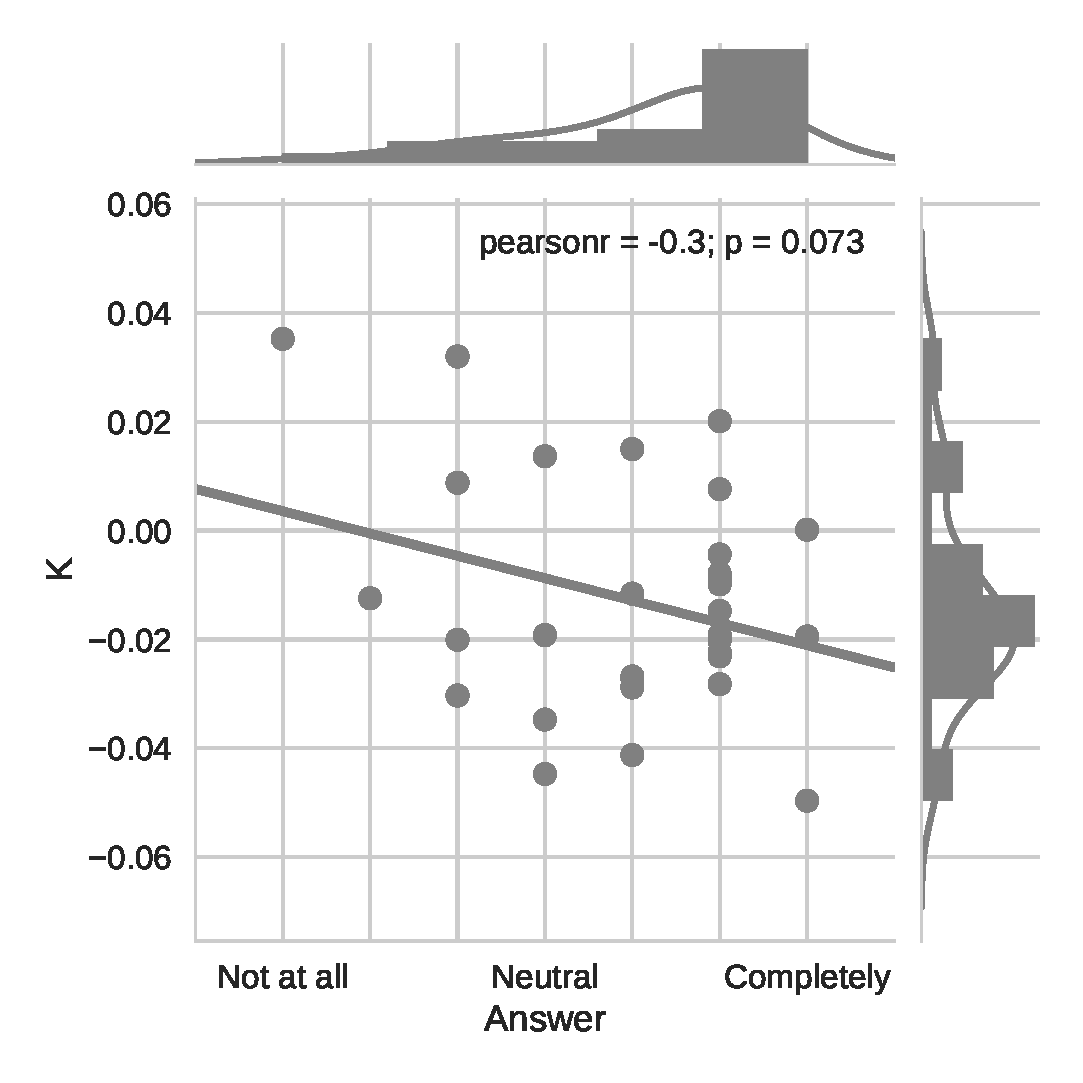
\includegraphics[trim={0cm 0cm 1cm 0cm},clip,width=.8\textwidth]{img/compelling}
		\caption{Correlation between subjective answers to the question \textit{the sense of playing in the remote environment was compelling} in the x-axis and objective metrics values}
		\label{subfig:compelling}
	\end{subfigure}
	\quad
	\begin{subfigure}[t]{.43\textwidth}
		\centering        
		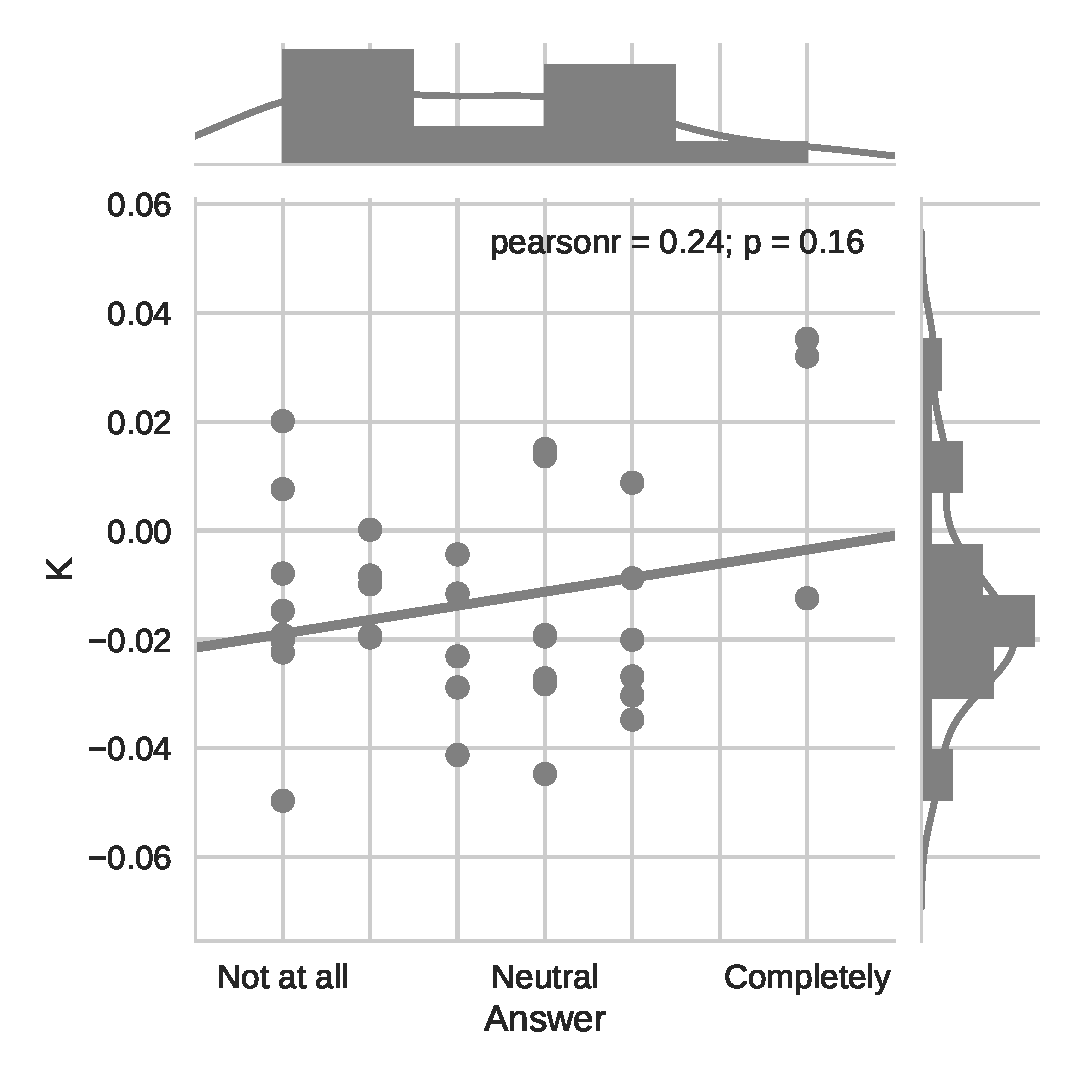
\includegraphics[trim={3cm 0cm 0cm 0cm},clip,width=.8\textwidth]{img/involvement}
		\caption{Correlation between subjective answers to the question \textit{the delay affected the sense of involvement} in the x-axis and objective metrics values}
		\label{subfig:involvement}
	\end{subfigure}
	\quad 
	\caption{Correlation between subjective answers in the x-axis and tempo slope $K$ in the y-axis.}\label{fig:ci}
	%	\vspace{-1em}
\end{figure*}  


\section{Results and discussion}\label{sec:discussion}
Though limited in the amount of involved people and performances, the experiments described in the previous section were helpful to start the discussion about the pedagogical applications of NMPs with musicians, and to collect useful comments and suggestions that will guide our investigation. 


\subsection{Objective, subjective and biological metrics}\label{subsec:metrics}
In the two experiments, we investigate the sense of presence and quality of performance of the couple of subjects in case of visual occlusion (co-presence experiment) and different network latency conditions (networked performance). The acquisition and evaluation was performed using subjective and objective metrics \cite{CIM2018}. 

With regard to the former, we used a post-experiment 27-item questionnaire divided in five main topics, such as \textit{Predictability and Interaction}, or \textit{Quality of the Music Performance}. After each phase of the networked experiments, we asked a subset of five questions to evaluate the impact of different latency conditions in the questionnaire.

With regard to the latter, we acquired the audio recordings of the networked performance, manually tracked the beat, extracted a BPM trend and computed a degree of acceleration/deceleration $K$  (\textit{tempo slope}) from it. Other metrics used in NMP literature include the pacing, the regularity or the imprecision of the performance \cite{RottondiOverview}.

It is interesting to observe the comparison between the subjectively-perceived quality of the performance and the  objective metrics computed from the corresponding audio recording. In Fig. \ref{fig:ci} we show the comparison with the answers to two quality-related questions, i.e., \textit{the sense of playing in the remote environment was compelling} (Fig. \ref{subfig:compelling}) and \textit{the delay affected the sense of involvement} (Fig. \ref{subfig:involvement}).

Due to the few samples we obtained, it is not possible to draw statistically-meaningful conclusions. The preliminary observations, however, show an interesting trend that we would like to investigate further. The musicians seem to be more compelled with the remote environment when the levels of $K$ were lower, i.e., when the tendency to slow down is more accentuated. Analogously, their sense of involvement in the performance show little correlation with the tempo trend. 

Two musicians, indeed, can easily keep the tempo by making one subject following the lead of the other, using a master-slave approach to cope with latency \cite{Carot07networkmusic}. In this case musicians would not improve their musical skills to interact with partners. From this results, we can infer that $K$ is not suitable to be used as an objective metrics of the subjective satisfaction of subjects. 

A first investigation in the project will be devoted to find a content-based metrics that is coherent with the pedagogical purposes of NMPs and suitable for providing a 
%We aim to extract such a metrics using content-based techniques, in order to provide a 
useful feedback for students.% and can guide our research for a more effective platform for NMP. 
This study will involve acquiring %to We may estimate metrics from the level of comfortability of the students during a lesson or a rehearsal. For this reason, we intend to acquire 
biometric signals to estimate the level of distress during the performance and to investigate whether the NMPs contribute to increase such level. 

\subsection{Auditory and visual feedback}
After the experiments, we asked musicians about the strategies they adopt for 
%From the co-presence experiment, we could observe different strategies of 
musical coordination and interpretation, which they report to be based on breathing signaling and communicative gestures to keep synchronization, especially for attacks and the duration of sustained notes. In the co-presence experiment, %is case, 
the no-sight condition deeply affected the expressiveness of the performance. In full visual occlusion, the performers relied mostly on acoustic cues to keep the tempo, with the apparent effect of an acceleration during the performance. 

\begin{figure}[b]
	\centering
	\begin{subfigure}[t]{.48\columnwidth}
		\centering        
		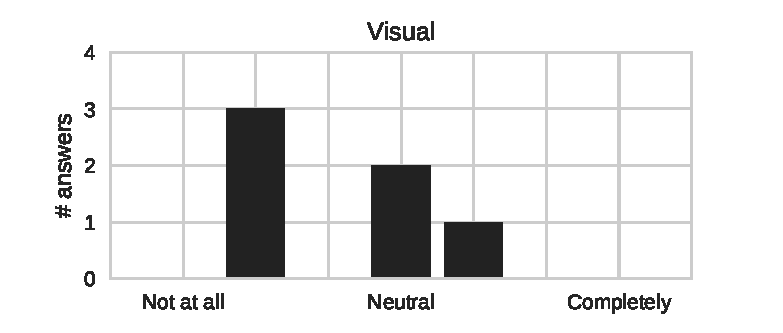
\includegraphics[trim={.5cm 0cm 1cm 0cm},clip,width=\textwidth]{img/Visual}
		\caption{Influence of the visual feedback}
		\label{subfig:visual}
	\end{subfigure}
	\begin{subfigure}[t]{.48\columnwidth}
		\centering        
		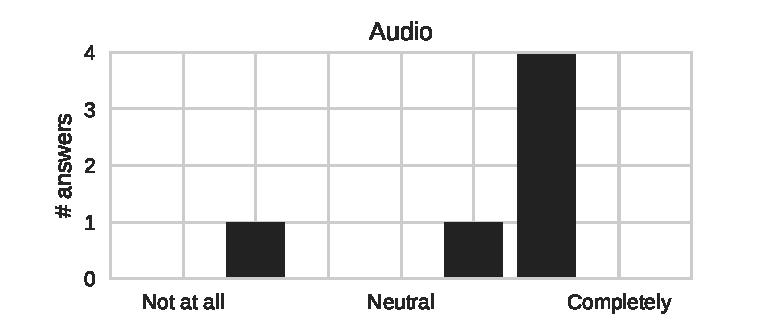
\includegraphics[trim={1.5cm 0cm 0cm 0cm},clip,width=\textwidth]{img/Audio}
		\caption{Influence of the auditory feedback}
		\label{subfig:audio}
	\end{subfigure}
	\quad 
	\caption{Histogram of the answers on the influence of visual and auditory feedback after the NMP experiment.}\label{fig:va}
	%	\vspace{-1em}
\end{figure}  

This aspect is also investigated in the remote performance by asking in the perceptual questionnaire how much the visual and auditory display quality interfered or distracted them from performing. In Fig. \ref{fig:va} we display a histogram of the answers in a 7-point likert scale. While the influence of the visual feedback is limited (Fig \ref{subfig:visual}), the auditory feedback is predominant for the performance.

During the time of free comments, the subjects explained that the video feedback was less relevant due to the low degree of synchronicity introduced by the latency, which led them to look less for a visual interaction with their partner. In order to translate these comments into requirements for a NMP tool, we need to assess the importance of visual and auditory interaction in performances and rehearsal. A level of auditory interaction can be estimated using a measure of asymmetry between the audio recordings of the two subjects, as computed in \cite{Chafe3}. With regard to visual interaction, we intend to acquire a video recording of the performance using cameras that capture when the subjects are watching at their partners on the screen. By annotating both intentional and saccadic movements, we aim at estimating whether a higher level of interaction between subjects corresponds to higher satisfaction in the performance and, possibly, how to design the visual and auditory feedback in our platform.
 
\subsection{Peripheral visual feedback}
In the previous subsection, we discussed the importance of visual feedback in co-presence and networked performances. During the co-presence experiment, we observed how performers where comfortable with blurred visual of their partners. They referred us that most of the information for synchronization is contained in the perception of motion from the partners, rather than in the full view.

In the networked experiment the subjects were placed in front of webcam and monitor in order to improve eye contact, as in \cite{duffy2017new}. Some participants of the networked performances commented that one of the reason of the influence of the visual feedback was the lower importance of direct visual interaction. In their typical disposition during rehearsal and performance they are placed in front of an audience rather than in front of each other and, therefore, mostly rely on peripheral vision for interacting.

As next steps, we intend to test the role of peripheral vision by trying different arrangement of video equipment and subjects during the NMPs. This involves to test different virtual environments and find the most promising for pedagogical purposes.  The most suitable arrangements may involve use multiple visual feedbacks, e.g., one frontal for eye contact and one for catching peripheral motion. This would mean dealing with multiple video streams, which demands a larger bandwidth. Reducing the demand in terms of bandwidth is nonetheless desirable in order to improve the spread of our tools. We intend to investigate on strategies to decrease the need of bandwidth.


\begin{figure}[t]
	\centering
	\begin{subfigure}[t]{.46\columnwidth}
		\centering        
		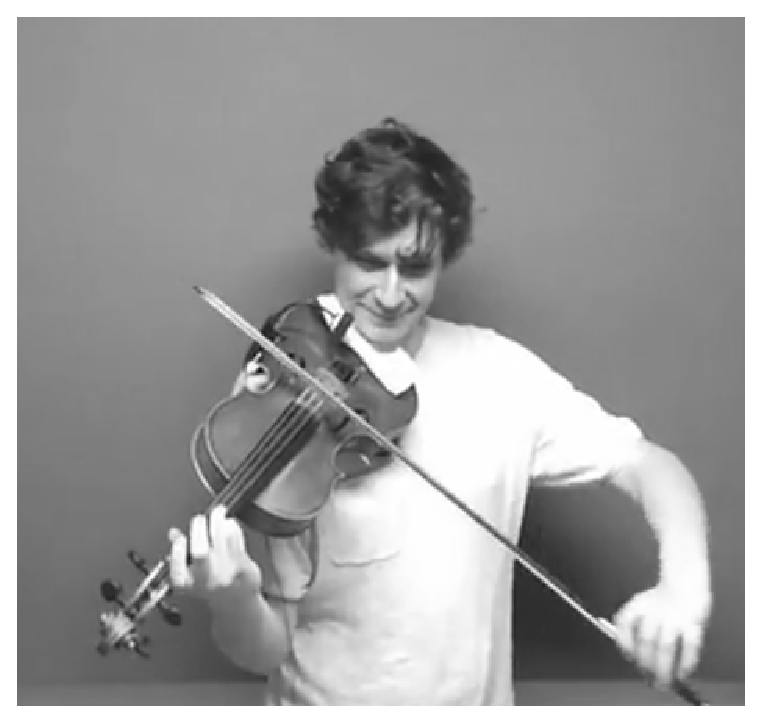
\includegraphics[trim={0cm 0cm 0cm 0cm},clip,width=\textwidth]{img/webcam}
		\caption{Normal view}
		\label{subfig:webcam}
	\end{subfigure}
	\quad
	\begin{subfigure}[t]{.46\columnwidth}
		\centering        
		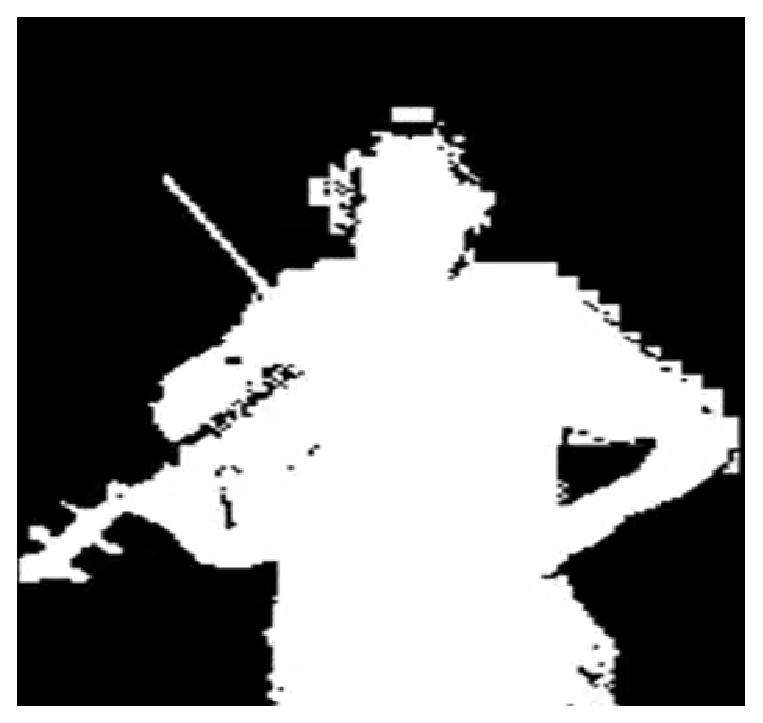
\includegraphics[trim={0cm 0cm 0cm 0cm},clip,width=\textwidth]{img/blob}
		\caption{BLOB view}
		\label{subfig:blob}
	\end{subfigure}
	\quad 
	\caption{Comparison between normal and BLOB view of a musician during a NMP.}\label{fig:wb}
	%	\vspace{-1em}
\end{figure}  


Both LOLA and Ultragrid implement several coding algorithm to reduce the bandwidth, while slightly increasing the processing time for coding/decoding the video streams \cite{drioli2013networked,holub2006high}. A higher saving would be to detect and transmits only the silhouette of the musicians as a binary large object (BLOB) \cite{camurri2010visual}. In Fig. \ref{fig:wb} we show a comparison between a normal take of a musician (Fig. \ref{subfig:webcam}) and a BLOB view (Fig. \ref{subfig:blob}).
Being a binary image, the BLOB view is extremely lighter, while keeping most of the information on the motion. As future directions, we intend to investigate whether the BLOB or other motion-related representations can effectively convey the information needed by musicians for rehearsing together. 


\subsection{Mono vs Stereo vs 3D Audio}
Monophonic audio acquisition and rendering is commonly used in NMPs \cite{CIM2018}. Some studies employ headphones to avoid audio loops \cite{RottondiFeature}, while others use monophonic speakers and echo-cancellation algorithms for avoiding feedbacks \cite{drioli2013networked}. 

The directionality of the sound is crucial %can be neglected for duo rehearsal or teacher-student lessons, but it is important 
in case of performances with many musicians, where it helps locating the sources and improving the ability to focus on the instruments separately. 

We intend to investigate the influence of sound directionality in NMPs by testing different audio conditions and verifying which one the musicians prefer. A first condition is to use panning with headphones and stereo speakers to place the sound sources. A second condition is to use binaural rendering for headphones and more accurate methods for the stereophonic location of the sounds. Lastly, we want to use an array of speakers in different arrangement to allow more accurate rendering of sound fields. 

It is also worth mentioning that it is not natural for musicians to wearing headphones during a performance, as they also affect their ability to hear their own sound. Moreover, to properly locate the sound sources in the virtual environment, the binaural rendering requires a proper head tracking algorithm to constantly update the location of sources with respect to the orientation of the listener \cite{Bonacina2016}.

There are further scenarios where a 3D acquisition of the sound field is required.  Most instruments have indeed a clear pattern of radiance and listening to them from different angles lead to sensible changes of the timbral properties \cite{CancliniAES}. In a teacher-student scenario, a teacher may be interested to have a richer information to assess the progress of their students. We aim to employ state-of-the-art techniques for the plenacoustic analysis and rendering, as in \cite{Canclini2015}.

%Even in case of a student-teacher lesson, a more directional acquisition may be required. Most instruments have indeed a clear pattern of radiance and listening to them from different angles lead to sensible changes of the timbral properties \cite{CancliniAES}. In this situation, a teacher may be interested to have a richer information to assess the progress of their students. We aim to employ state-of-the-art techniques for the plenacoustic analysis and rendering, as in \cite{Canclini2015}.

\subsection{Matching acoustics of environments}
In the networked experiment we did not take the influence of room acoustics for the performance into consideration. In other experiments, the performers play in acoustically insulated and semi-anechoic rooms to remove this influence \cite{RottondiFeature}. Musicians have difficulty playing in semi-anechoic rooms, as the perceived timbre of instruments change dramatically making hard for them to recognize the quality of their performance \cite{Woszczyk2009}.

In real-case scenarios, it is likely that musicians are going to perform over network from two acoustically-different environments. In this case, they would listen to their own sound colored by their environment and receive their partner audio signal from a different acoustic, creating a misalignment between the two environments.

In future work, we want to take the effect of environment acoustic into account by testing different combinations of real rooms' acoustics and synthetically-processed acoustics~\cite{Boucher15}. This will help us understanding if musicians require techniques to address the issue of different acoustic environments for having a realistic performance. These techniques may involve to first blindly assess the acoustic conditions of the two environments and then de-convolve the partner's audio stream \cite{CancliniRoom}.



\subsection{Measure for latency compensation and virtual conductor}
One of the main factor investigated in the NMP literature was the influence of network latency in the quality \cite{RottondiOverview,drioli2013networked}, as we also did in the networked experiment. The new 5G network is showing promising results for enabling low-latency connections, that may enable NMPs applications even for generic users \cite{uk5G}. Nevertheless, a certain amount of latency is likely to be present for NMPs using general purpose hardware and connections. 

For this reason, researchers have been developing strategies to cope with the latency. In \cite{Carot07networkmusic} the authors identify a set of strategies such as the laid-back approach, which involves for a musician to play slightly behind the beat, and the delayed feedback approach, which involves to equip one of the musician with a delayed feedback of their own sound in order to synchronize it with their partners sound. The presence of a conductor has also been shown to increase the tolerance to delay, thanks to the shared cue provided to the performers \cite{Olmos2009}.

In the project, we aim to develop algorithms that help musicians compensating for the delay. We plan to use a beat tracker to dynamically track the rhythm of the performance of the musicians, as in \cite{Goto2010}, and provide it in advance to musicians. This will allow musicians to follow a virtual conductor, similarly to what proposed in \cite{conductor2008}.


\section{Conclusion}\label{sec:conclusion}
%This part presents the key findings in substance. Avoid simple enumeration of the following material. It is desirable to provide a link to existing articles and grants. 

Using Networked Music Performances for pedagogical scenarios require a deep investigation on the topic to find metrics, factors and aspects that may help musicians to improve their musical skills.

In this paper, we introduced a framework for conducting perceptual experiments to continue this investigation for the purposes of the project InterMUSIC. We then presented two experiments conducted using the framework and the preliminary results that we observed.

Starting from this results, we described the areas of investigation that we intend to follow, with the final goal of developing a platform for NMPs in pedagogical scenarios that also work with general-purpose hardware.

Beyond this areas, in future work we intend to further develop the formalization of the framework into an ontology, which will be integrated in the NMP tools, in order to collect and analyze a number of semantically-annotated rehearsal or lessons \cite{Kolazi2013}. 

\section*{Acknowledgment}
%\section{Acknowledgment}
%The work described in this paper is part of the project InterMUSIC, 
This study was conducted for the InterMUSIC project,
which received the financial support of the Erasmus+ National Agency under the KA203 Strategic Partnership action under grant number: 2017-1-IT02-KA203-036770.

The authors would like to thank the participants of the  pilot tests for their effort and their availability to be contacted for further experiments. 

\begin{thebibliography}{6}


\bibitem{Lazzaro2001}
J.Lazzaro and J.Wawrzynek, ``A case for network musical performance'', in \emph{Proc. NOSSDAV Workshop}, Jun. 2001, pp. 157--166. 


\bibitem{IorwerthNMP2015}
M. Iorwerth, D. Moore and D. Knox, ``Challenges of using Networked Music Performance in education'', in  \emph{Proc. AES Conference}, Aug. 2015, pp. 157--166. 


\bibitem{MIDItoolbox}
T. Eerola and P. Toiviainen, \emph{MIDI Toolbox: MATLAB Tools for Music Research}, Finland: University of Jyv{\"a}skyl{\"a},  2004.

\bibitem{MOOCS}
N. Lushnikova, P. Chintakayala and A. Rodante, ``Massive Open Online Courses from Ivy League Universities: Benefits and Challenges for Students and Educators'' \emph{in proc. of the XI International Conference “Providing continuity of content in the system of stepwise graduate and postgraduate education}, Nov. 2012

\bibitem{Kolazi2013}
\c{S}. Kolozali and M. Barthet and G. Fazekas and M. Sandler, ``Automatic Ontology Generation for Musical Instruments Based on Audio Analysis'', in \emph{IEEE Transactions on Audio, Speech, and Language Processing}, Oct. 2013, pp. {2207--2220}
%	year={2013}, 
%	volume={21}, 
%	number={10}, 

\bibitem{camurri2010visual}
A. Camurri and T. Moeslund, Chap. ``Visual gesture recognition'' in \emph{Musical Gestures: Sound, Movement, and Meaning}, Edited by R. I. God{\o}y, and M. Leman, Routledge, 2010

\bibitem{Canclini2015}
A. Canclini, L. Mucci, F. Antonacci, A. Sarti, S. Tubaro, ``A Methodology for estimating the ratiationpattern of a violin during the performance'' \emph{in Proc. of the European Signal Processing Conference (EUSIPCO)}, 2015

\bibitem{Olmos2009}
A. Olmos, M. Brul\'{e}, N. Bouillot, M. Benovoy, J. Blum, H. Sun, N. W. Lund, and J. R. Cooperstock, ``Exploring the role of latency and orchestra placement on the networked performance of a distributed opera'' \emph{in 12th annual international workshop on presence}, 2009

\bibitem{Goto2010}
M. Goto, ``An Audio-based Real-time Beat Tracking System for Music With or Without Drum-sounds'' in \emph{Journal of New Music Research}, 30:2, pp. 159-171, 2010 

\bibitem{conductor2008}
A. Nijholt, D. Reidsma, R. Ebbers and M. ter Maat, ``The Virtual Conductor: Learning and Teaching about Music, Performing, and Conducting'', in \emph{proc. of the IEEE International Conference on Advanced Learning Technologies}, 2008

\bibitem{duffy2017new}
S. Duffy, and P. Healey, ``A new medium for remote music tuition'', in \emph{Journal of Music, Technology \& Education}, 2017, pp 5--27

\bibitem{uk5G}
UK 5G Innovation Network, Video: World's First 5G Distributed Music Concert, Web: https://uk5g.org/discover/read-articles/video-worlds-first-5g-distributed-music-concert/

\bibitem{CancliniAES}
A. Canclini, L. Mucci, F. Antonacci, A. Sarti and S. Tubaro, ``Estimation of the radiation pattern of a violin during the performance using plenacoustic methods'' \emph{in Audio Engineering Society Convention 138}

\bibitem{CancliniRoom}
A. Canclini, D. Marković, L. Bianchi, F. Antonacci, A. Sarti, S. Tubaro, ``A geometrical approach to room compensation for sound field rendering applications'' \emph{in Proc. of the European Signal Processing Conference (EUSIPCO)}, 2014

\bibitem{Bonacina2016}
L. Bonacina, A. Canclini, F. Antonacci, M. Marcon, A. Sarti, S. Tubaro, ``A low-cost solution to 3D pinna modeling for HRTF prediction'' in \emph{Proc. of the IEEE International Conference on Acoustics, Speech and Signal Processing (ICASSP)}, 2016

%	volume={10},
%	number={1},
%	pages={5--29},
%	year={2017},
%	publisher={Intellect}

%	m
%	\bibitem{Cover}
%	\textit{(Example for books)} T.M.Cover and J.A. Thomas, \emph{Elements of Information Theory}. New York: Wiley, 1991.
%	
%	\bibitem{Dobrushin}
%	\textit{(Example for articles)} R.L. Dobrushin, ``Optimum information transmission through a channel with unknown parameters'',  \emph{Radiotech.Electron.}, vol.4, Dec.1959, pp. 1951-1956.
%	
%	\bibitem{Blachman}
%	\textit{(Example for articles)} N.M. Blachman, ``Communication as a game'', \emph{in Proc. WESCON Conf.}, Aug. 1957, pp. 61-66.
%	
%	\bibitem{IEEE}
%	\textit{(Example for web-links)} IEEE official website, Manuscript Templates for Conference Proceedings, Web: http://www.ieee.org/conferences\_events/conferences/publishing/templates.\newline html.
%	
%	\bibitem{Elissa}
%	\textit{(Example for unpublished references)} K. Elissa, ``Title of paper if known'', unpublished.
%	
%	\bibitem{Nicole}
%	\textit{(Example for references have been accepted for publication)} R. Nicole, ``Title of paper with only first word capitalized'', J. Name Stand. Abbrev., in press.
%	
% INTRO
\bibitem{barbosa2003displaced}
A. Barbosa, ``Displaced soundscapes: A survey of network systems for music and sonic art creation'',
\emph{Leonardo Music Journal},
pp. 53--59,2003,MIT Press
%
\bibitem{RottondiOverview}
C. Rottondi, C. Chafe, C. Allocchio, and A. Sarti
``An Overview on Networked Music Performance Technologies'', \emph{IEEE Access},4,2016
%
\bibitem{Lakiotakis}
E. Lakiotakis, C. Liaskos, X. Dimitropoulos, ``Improving networked music performance systems using application-network collaboration'', \emph{Concurrency and Computation: Practice and Experience},Wiley Online Library, 2018

\bibitem{RottondiFeature}
C. Rottondi, M. Buccoli, M. Zanoni, D. Garao,  G. Verticale and A. Sarti, ``Feature-Based Analysis of the Effects of Packet Delay on Networked Musical Interactions'', \emph{Journal of the Audio Engineering Society}, 63(11), 864-875.
% Chafe clapping experiments
\bibitem{Chafe3}
C. Chafe, J-P. Caceres, M. Gurevich, ``Effect of temporal separation on synchronization in rhythmic performance'',
\emph{Perception}, 39(7): 982-992, 2010
%
\bibitem{Chafe2}
C. Chafe and M. Gurevich, ``Network Time Delay and Ensemble Accuracy: Effects of Latency, Asymmetry'', \emph{Proc. of the AES 117th Conf.}, SF, 2004
%
\bibitem{Chafe1}
C. Chafe, M. Gurevich, et al. ``Effect of Time Delay on Ensemble Accuracy''
\emph{Proc. 2004 Intl. Soc. Musical Acoustics}, Nara, 2004
% BArbosa

\bibitem{Carot07networkmusic}
E. Car\^ot and C. Werner, ``Network music performance - problems, approaches and perspectives'',
\emph{International School of new Media, Institute of Telematics, University of Lübeck. Music in the Global Village - Conference} ,2007
%

\bibitem{gurevich2011ambisonic}
M. Gurevich, D. Donohoe and S. Bertet, ``Ambisonic Spatialization for Networked Music Performance'', \emph{International Community for Auditory Display}, 2011
% reverberation studies

\bibitem{carot2009towards}
A. Car{\^o}t, C. Werner and T. Fischinger, ``Towards a comprehensive cognitive analysis of delay-influenced rhythmical interaction'', \emph{ICMC}, 2009
%
\bibitem{FarnerReverb}
S. Farner, A. Solvang, A. S{\ae}b{\o} and Peter Svensson, A. Car{\^o}t, C. Werner and T. Fischinger, ``Ensemble hand-clapping experiments under the influence of delay and various acoustic
environments'',\emph{Journal of the Audio Engineering Society}, 57(12), pp 1028--1041, 2009
% LOLA

\bibitem{drioli2013networked}
C. Drioli, C. Allocchio, and N. Buso,
``Networked performances and natural interaction via LOLA: Low latency high quality A/V streaming system'',
\emph{Information Technologies for Performing Arts, Media Access, and Entertainment}, Springer, 2013
pp.240--250,
%Ultragrid
\bibitem{holub2006high}
P. Holub, L. Matyska, M. Li{\v{s}}ka, L. Hejtm{\'a}nek, J. Denemark, T. and Rebok, A. Hutanu, R. Paruchuri, J. Radil, and E. Hladk{\'a}
``High-definition multimedia for multiparty low-latency interactive communication'',
\emph{Future Generation Computer Systems},
22(8),
pp.856--861,
2006,
Elsevier
%Jacktrip
\bibitem{CaceresJacktrip}
J.-P. C\'{a}ceres, C. Chafe, ``JackTrip: Under the Hood of an Engine for Network Audio'', \emph{Proceedings of International Computer Music Conference}, Montreal, 2009. 

\bibitem{CIM2018}
S. Delle Monache, M. Buccoli, L. Comanducci, A. Sarti, G. Cospito, E. Pietrocola and F. Berbenni, ``Time is not on my side: network latency, presence and performance in remote music interaction.'' \emph{Proceedings of the XXII Colloquium on Musical Informatics (CIM)}, Udine,20-23 November, 2018.
%
\bibitem{Markovic2013} 
D. Markovic and F. Antonacci and A. Sarti and S. Tubaro, ``Soundfield Imaging in the Ray Space'',
\emph{IEEE Transactions on Audio, Speech, and Language Processing}, 
21(12), 
pp. 2493-2505, 2013
%
\bibitem{bianchi2016}
L. Bianchi, F. Antonacci, A. Sarti, S. Tubaro,
``Model-Based Acoustic Rendering based on Plane Wave Decomposition'',
\emph{Applied Acoustics},
Elsevier,
2016(104),
pp. 127--134
% Saccadic movements annotation
\bibitem{vandemoortele2018gazing}
S. Vandemoortele, K. Feyaerts, G. De Bi{\`e}vre, M. and Reybrouck, G. Br{\^o}ne, T. De Baets,
``Gazing at the partner in musical trios: a mobile eye-tracking study'',
\emph{Journal of Eye Movement Research}, 
Vol.11(2),2018
pp.6
% Biometric signal monitoring
\bibitem{Yoshie2009}
Yoshie, Michiko
and Kudo, Kazutoshi
and Murakoshi, Takayuki
and Ohtsuki, Tatsuyuki, ``Music performance anxiety in skilled pianists: effects of social-evaluative performance situation on subjective, autonomic, and electromyographic reactions'',
\emph{Experimental Brain Research},
vol.199(2),22 Aug.2009,pp.117
%
\bibitem{Woszczyk2009}
Wieslaw Woszczyk and William Martens, ``Evaluation of virtual acoustic stage support for musical performance'', \emph{Journal of the Acoustical Society of America}, Vol. 123(5), 2008, pp. 3089
%
\bibitem{Boucher15}
Matthew Boucher, David Pelegrin-Garcia, Bert Pluymers, and Wim Desmet, ``Auralization as a tool for evaluating an acoustical instrument'', \emph{Proc. of the Third Vienna Talk on Music Acoustics}, 16–19 Sept. 2015, University of Music and Performing Arts Vienna, pp. 19
%	
%	\bibitem{Cover}
%	\textit{(Example for books)} T.M.Cover and J.A. Thomas, \emph{Elements of Information Theory}. New York: Wiley, 1991.
%	
%	\bibitem{Dobrushin}
%	\textit{(Example for articles)} R.L. Dobrushin, ``Optimum information transmission through a channel with unknown parameters'',  \emph{Radiotech.Electron.}, vol.4, Dec.1959, pp. 1951-1956.
%	
%	\bibitem{Blachman}
%	\textit{(Example for articles)} N.M. Blachman, ``Communication as a game'', \emph{in Proc. WESCON Conf.}, Aug. 1957, pp. 61-66.
%	
%	\bibitem{IEEE}
%	\textit{(Example for web-links)} IEEE official website, Manuscript Templates for Conference Proceedings, Web: http://www.ieee.org/conferences\_events/conferences/publishing/templates.\newline html.
%	
%	\bibitem{Elissa}
%	\textit{(Example for unpublished references)} K. Elissa, ``Title of paper if known'', unpublished.
%	
%	\bibitem{Nicole}
%	\textit{(Example for references have been accepted for publication)} R. Nicole, ``Title of paper with only first word capitalized'', J. Name Stand. Abbrev., in press.
%	

\end{thebibliography}

\end{document}